\documentclass[12pt]{beamer}

% INCLUDE GRAPHICS
\usepackage{graphicx}

% TABLES
\newcommand{\ra}[1]{\renewcommand{\arraystretch}{#1}} % spaces in tables
\usepackage{booktabs}   % Allows the use of \toprule, \midrule and \bottomrule in tables for horizontal lines

% FONTS
% PdfLatex
% \usepackage[T1]{fontenc}
% \usepackage{pgf}
% \logo{\pgfputat{\pgfxy(-1,-0.435)}{\pgfbox[center,base]{
\includegraphics[width=1.2cm,natwidth=610,natheight=642]{KUNATLogo.pdf}}}}

% FONTS
% xelatex
\usepackage{fontspec}
% \fontspec[Path=../fonts/,]{
%     UprightFont = *-regular,
%     ItalicFont = *-italic,
%     Boldfont = *-bold
% }

% NOTE
% Add fonts to ~/.fonts for this to work
% \setsansfont{TeX Gyre Heros}
% \setsansfont{TeX Gyre Heros Cn}
% \setsansfont{Liberation Sans}
\setsansfont{Muli}
% \setsansfont{Helvetica Neue}

% Monospaces font
\setmonofont{Monaco}

% Use serif for Math environments
\usefonttheme[onlymath]{serif}

% TODO Use mono fonts

% CODE
\usepackage{listings} % Code block (source code) \begin{lstlisting}
\lstset{
    language=Python,                        % Code langugage
    commentstyle=\color{gray},              % Comments font
    basicstyle=\scriptsize\ttfamily,             % Code font, Examples: \footnotesize, \ttfamily
    keywordstyle=\bfseries\color{blue},
    stringstyle=\color{orange},
    numbers=left,                           % Line nums position
    numberstyle=\tiny,                      % Line-numbers fonts
    stepnumber=1,                           % Step between two line-numbers
    numbersep=5pt,                          % How far are line-numbers from code
    numbers=none,
    frame=lines,                             % A frame around the code
    rulecolor=\color{gray},
    tabsize=4,                              % Default tab size
    captionpos=b,                           % Caption-position = bottom
    breaklines=true,                        % Automatic line breaking?
    breakatwhitespace=false,                % Automatic breaks only at whitespace?
    showspaces=false,                       % Dont make spaces visible
    showstringspaces=false,                 % Dont make spaces visible in strings
    showtabs=false,                         % Dont make tabls visible
    belowskip=5pt,
    morekeywords={range, xrange},
    backgroundcolor=\color{white}
    % emph={[2]root,base}
    % morekeywords={one,two,three,four,five,six,seven,eight,
}

\newcommand{\code}[1]{{\small\ttfamily #1}} % \code{inline code}

%
% COLORS
%
\definecolor{kugreen}{RGB}{50,93,61}

\definecolor{orange}{RGB}{255,127,0}
\definecolor{green}{RGB}{0,153,51}
\definecolor{blue}{RGB}{3,115,187}
\definecolor{red}{RGB}{221,17,68}
\definecolor{gray}{RGB}{55,55,55}
\definecolor{black}{RGB}{0,0,0}

\definecolor{offwhite}{RGB}{249,242,215}
\definecolor{foreground}{RGB}{23,23,23}
\definecolor{background}{RGB}{255,255,255}
\definecolor{subtitle}{RGB}{102,255,204}
\definecolor{hilight}{RGB}{102,255,204}
\definecolor{vhilight}{RGB}{255,111,207}
\definecolor{lolight}{RGB}{155,155,155}


%
% BEAMER STYLE COLORS
%
\setbeamercolor{titlelike}{fg=black}
\setbeamercolor{subtitle}{fg=blue}
\setbeamercolor{institute}{fg=gray}
\setbeamercolor{normal text}{fg=foreground,bg=background}
\setbeamercolor{item}{fg=foreground} % color of bullets
\setbeamercolor{subitem}{fg=gray}
\setbeamercolor{itemize/enumerate subbody}{fg=gray}

\setbeamerfont{itemize/enumerate subbody}{size=\footnotesize}
\setbeamerfont{itemize/enumerate subitem}{size=\footnotesize}

\setbeamerfont{footnote}{size=\tiny}

\setbeamersize{text margin left=10pt}
\setbeamersize{text margin right=10pt}
\setbeamersize{sidebar width right=0pt}
\setbeamersize{sidebar width left=0pt}

%
% REMOVES THE NAVIGATION BAR
%
\beamertemplatenavigationsymbolsempty


% BEAMER TEMPLATES


%
% BEAMER BACKGROUND
%
\usebackgroundtemplate{

    \rule{0pt}{0.97\paperheight}%
    \hspace*{1.15\paperwidth}%
    \makebox[0pt][r]{%
        
\includegraphics[width=100pt,natwidth=610,natheight=642]{KUNATLogo.pdf}
    }

}


%
% BEAMER HEADLINE
%
\setbeamertemplate{headline}{}


%
% BEAMER TITLE
%
\setbeamertemplate{frametitle}
{
    \begin{centering}
    \insertframetitle\par
    \end{centering}
}


%
% BEAMER FOOTER
%
\setbeamertemplate{footline}[text line]
{%
    \vbox{%
        \insertvrule{0.5pt}{kugreen}

        \vspace{2pt}

        \strut{
        % \rmfamily\itshape
        \expandafter\insertshorttitle
        \expandafter\insertauthor
        \insertshortinstitute
        }
        \hfill\strut{
        }
        \hfill\strut{
            \insertframenumber\,/\,\inserttotalframenumber
        }

        \vspace{1pt}
    }
}


%
% TITLE PAGE
%
% \setbeamertemplate{title page}
% {
%     % Remove beamer background
%     \setbeamertemplate{background}{}
% 
%     \begin{beamercolorbox}[center]{beamer color}
% 
%         {
%             \huge
%             \color{kugreen}
%             \inserttitle
%         }
%         \bigskip
%         \bigskip
% 
%         % 
\includegraphics[width=2cm]{KUNATLogo}
% 
%         \bigskip
%         {
%             \bf
%             \rmfamily
%             {\large \insertauthor}
%         }
% 
%         \smallskip
%         {
%             \rmfamily
%             \footnotesize
%             \insertinstitute
%         }
% 
%         {
%             \rmfamily
%             \footnotesize
%             \insertdate
%         }
% 
%     \end{beamercolorbox}
% 
%     % Do not count the title page
%     \addtocounter{framenumber}{-1}
% }

\usepackage{amsmath}
\usepackage{animate}
\usepackage{soul}

\title[]{Week 4\\Molecular Statistics}


\institute[, University of Copenhagen]{C315B\\ Department of Chemistry \\ University of Copenhagen}

\author[J. C. Kromann]{Jimmy Charnley Kromann}

\date{
    \code{\scriptsize help: jimmy@charnley.dk}
}




% ===============
% begin slides
% ===============


\begin{document}

{
\usebackgroundtemplate{}
\begin{frame}[plain]
    \titlepage
    \addtocounter{framenumber}{-1}
\end{frame}
}

% please stop that overview stuff jimmy
% \begin{frame}[fragile]
%
%     \frametitle{Week 4, Overview}
%
%     \begin{itemize}
%
%         \item anaconda / compile
%
%         \item modules
%
%         \item Numpy Tricks
%
%         % \item Diffusion, random walk Monte Carlo
%
%     \end{itemize}
%
% \end{frame}
%

\begin{frame}[fragile]
% Anaconda includes over 100 prepackaged scientific packages
    \frametitle{Interpret Vs. Compiling}

    \centering

    Today we use anaconda. Why?

 
\includegraphics[width=0.7\textwidth]{images/anaconda.png}

% \begin{lstlisting}
% @jit()
% def force(R, box_width, eps):
%     for i in range(n_part):
%         for j in range(n_part):
%             if i > j:
%                 X  = R[0, j] - R[0, i]
%                 Y  = R[1, j] - R[1, i]
%                 X  -= box_width * np.rint(X/box_width)
%                 Y  -= box_width * np.rint(Y/box_width)
%                 ...
% \end{lstlisting}
%
%     becomes
%
% \begin{lstlisting}
% 0100101001100100101010000010001110
% 1110101001010101001010100101000111
% 0100100100110101100101001101010101
% \end{lstlisting}
%

    {
        \scriptsize
        picture source: https://www.continuum.io/downloads}

\end{frame}


\begin{frame}[fragile]

    \frametitle{Interpret Vs. Compiling}
%An intepret language is run "on the fly" - as the program is run each bit of the program is "translated" into native machine language - a compiled language needs to be compiled before it can be run - this oftens makes the program faster
\begin{center}
 
\includegraphics[width=0.4\textwidth]{images/numba.png}
\end{center} 
\end{frame}
 
\begin{frame}[fragile]

    \frametitle{Interpret Vs. Compiling}
    
\begin{lstlisting}
@jit()
def force(R, box_width):
    for i in range(n_particles):
        for j in range(n_particles):
            if i>j:
                rij = distance(x_positions[i],
                energy += 4*(1.0/rij**12 - 1.0/
                fx = -48*(x_positions[j] - x_po
                fy = -48*(y_positions[j] - y_po
                x_forces[i] = x_forces[i] + fx
                y_forces[i] = y_forces[i] + fy
\end{lstlisting}

    becomes

\begin{lstlisting}
01001010011001001010100000100011101110101001010101001010100101000
11101001001001101011001010011010101011110100100100110101100101001
\end{lstlisting}


\end{frame}


\begin{frame}[fragile]

    \frametitle{Making modules}

my\_functions.py
\begin{lstlisting}
def square(x):
    return x**2

\end{lstlisting}

\bigskip

anotherfile.py
\begin{lstlisting}a
import my_fuctions
print my_functions.square(2)
\end{lstlisting}

\end{frame}


\begin{frame}[fragile]

    \frametitle{Numpy Tricks}


    \begin{columns}[t]

        \column{0.5\linewidth}

            array intialization

            \begin{itemize}
                \item \code{np.array(list)}

                \item \code{np.zero((3,3))}

                \item \code{np.arange(5)}

            \end{itemize}

            %"views"

        \column{0.5\linewidth}


            array mathematics

            \begin{itemize}
                \item \code{np.sqrt(a)}
                \item \code{ += }
                \item \code{A*A}
            \end{itemize}

            array methods

            \begin{itemize}
                \item \code{mean}
                \item \code{sum}
                \item \code{prod}
                \item \code{min / max}
                \item \code{argmin / argmax}
            \end{itemize}

    \end{columns}

\end{frame}


% \begin{frame}[fragile]
% 
%     \frametitle{Diffusion}
% 
%     \begin{columns}[t]
% 
%         \column{0.5\linewidth}
%             \centering
% 
%             
\includegraphics[width=0.4\textwidth]{ink.jpg}
% 
%         \column{0.5\linewidth}
% 
%             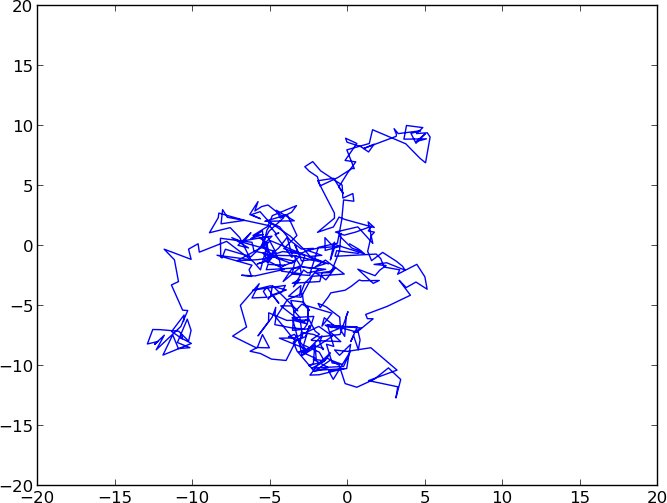
\includegraphics[width=0.8\textwidth]{one_particle.jpg}
% 
%     \end{columns}
% 
%     \bigskip
%     \bigskip
% 
%     Monte Carlo - Random walk (no interaction)
%     \begin{align*}
%         R_{x,i}(t+dt) = R_{x,i}(t) + \mathrm{random()}\\
%         R_{y,i}(t+dt) = R_{y,i}(t) + \mathrm{random()}
%     \end{align*}
% 
% \end{frame}


% \begin{frame}[fragile]
% 
%     \frametitle{Diffusion}
% 
%     Fick's second law of diffusion
%     \begin{align*}
%         \frac{\partial \phi }{\partial t} = D \frac{\partial^2 \phi }{\partial x^2}
%     \end{align*}
% 
%     Solution: a gauss-function
%     \begin{align*}
%         \phi(x, t) = \frac{1}{\sqrt{2 \pi \sigma^2}} \exp \left (-\frac{x^2}{2 \sigma^2} \right )
%     \end{align*}
% 
%     \begin{itemize}
%         \item $\sigma = \sqrt{2 D t}$ or $D = \sigma^2/2t$
%         \item in 3 dimensions, $x^2$ becomes $x^2 + y^2 + z^2$
%     \end{itemize}
% 
%     if we can simulate $\phi(x,t)$ we can calculate $D$.
% 
% \end{frame}
% 

\begin{frame}[fragile]

    \frametitle{Bubblesort}
 \begin{center}
 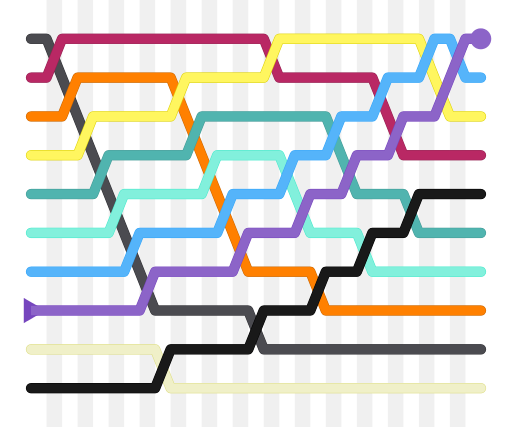
\includegraphics[scale=0.4]{images/Bubblesort-edited-color.svg.png}
 \end{center}

\end{frame}

\begin{frame}[fragile]

    \frametitle{The exercise, in Numpy}

    Velo-Verlet, Update positions, the Numpy way
    \begin{align*}
        R_x(t + dt) = R_x(t) + dt\ V_x(t) + 0.5\ dt^2\ A_x(t) \label{eq:position_x}
    \end{align*}


    \bigskip

\begin{lstlisting}
for n in range(n_steps):
    for i in range(n_particles):
        X[i] = X[i] + dt*Vx[i] + 0.5*dt*dt*Fx[i]
\end{lstlisting}

becomes

\begin{lstlisting}
for n in range(n_steps):
    X += dt*Vx + 0.5*dt*dt*Fx
\end{lstlisting}

\end{frame}






%%%%%%%%%%%%%%%%%%%%%%%%%%%%%%%%%%%%%%%%%%%%%%%%%%%%%%%%%%%%%%%%%%%%%%
%% END FRAMES
%%%%%%%%%%%%%%%%%%%%%%%%%%%%%%%%%%%%%%%%%%%%%%%%%%%%%%%%%%%%%%%%%%%%%%

\end{document}

